%%%%%%%%%%%%%%%%%%%%%%%%%%
%                                                        %
%                Graphical Representation                %
%                                                        %
%%%%%%%%%%%%%%%%%%%%%%%%%%

\labChapter{}{Graphical Representation of Experimental Data}

From an examination of the tabulated values of a number of measurements of related quantities, it is often difficult to grasp the relationships existing between the numbers. A method widely used to discover such relationships is the graphical method, which gives a pictorial view of the results and makes it possible to interpret the data by a quick glance.

% Independent and Dependent Variables
\section{Independent and Dependent Variables}

In any experimental study of cause and effect the aim is to vary just one condition at a time (the cause) and to observe the corresponding values of another quantity (the effect), which is suspected of being related to the first. The existing relationship is most easily interpreted from the graph if the first of these quantities, the independent variable, is plotted on the abscissa scale ($x$-axis), and the dependent variable is plotted on the ordinate scale ($y$-axis). For example,
\[
y = f(x)
\]
means that for each value $x$, the independent variable, there is a corresponding value of $y$, or, $y$ is a function of $x$.

Graphs should have the following features:
\begin{itemize}
\item[$\triangleright$] Axes tick marks and axis labels indicating the numerical scale  of the quantity,
\item[$\triangleright$] Axes titles with the name of the quantity and the units,
\item[$\triangleright$] A descriptive graph title,
\item[$\triangleright$] Points should not be joined by lines and there is no need to label them with the actual values, and
\item[$\triangleright$] If possible, the full scale should be visible and axes should intersect at $(0,0)$.
\end{itemize}
An example of how a graph should look is shown in Fig.~\ref{fig:graph}.

\begin{figure}%[htbp] %  figure placement: here, top, bottom, or page
  \begin{center}
    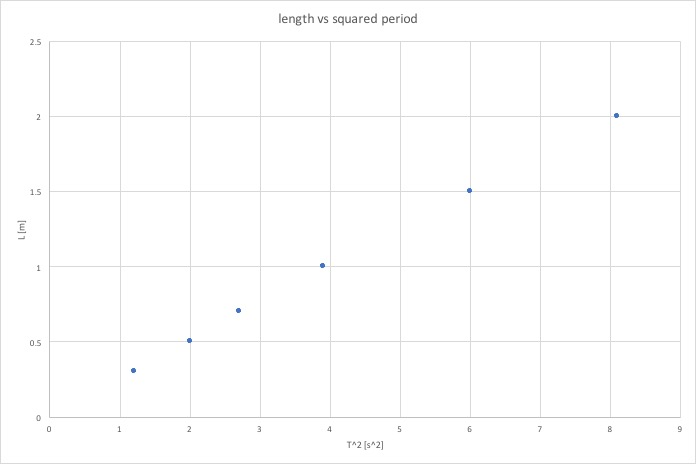
\includegraphics[width=4in]{IntroductionFigures/graph.jpg}
  \end{center}
  \caption{Example of a graph for the pendulum experiment showing the length as a function of the period squared.}
  \label{fig:graph}
\end{figure}

% Producing Graphs
\section{How to Produce Graphs}

There are many ways to produce graphs and just as many computer programs that will aid in the representation of data. This section will give simple instructions on how to make data graphs, using Excel.

\begin{itemize}
\item[$\triangleright$] Using a spreadsheet, it's easiest if you create a separate data table for each graph you want to make. By default Excel expects the first column of the table to be the values for the $x$-axis and the second column the values for the $y$-axis.
\item[$\triangleright$] Highlight \textit{both} columns and select \textbf{Charts} from the toolbar menu. Select the \textbf{Scatter} type and Excel will automatically produce the graph in your spreadsheet.
\item[$\triangleright$] You need to add labels and units to both axes by selecting the option \textbf{Axis Titles} in Excel and then edit the title by clicking on it.
\item[$\triangleright$] Very often you want to add a line-of-best-fit to your Excel graph. To do so follow the steps below:
  \begin{enumerate}
  \item In your graph, right-click (in Windows) or CTRL-click (on Mac) on one of the data points. This will open a pop-up menu. In this menu select \textbf{Add Trendline}. This will open a window with several items related to best-fit-lines and curves.
  \item Select the type of line you would like to add from the \textbf{Type} menu. If you want a straight line select \textbf{Linear}, for a polynomial (e.g.\ a parabola) select \textbf{Polynomial} and then the order will give the highest exponent (for a parabola the order would need to be a \textbf{2}).
  \item In the \textbf{Options} menu you can select two important options for the trend line:
    \begin{itemize}
    \item The \textbf{Set Intercept = \textit{value}} option will force the trendline to go through the point (0,\textit{value}). This is useful if you know that your curve is supposed to go through the origin. In this case set $\mbox{\textit{value}} = 0$ (the default value in Excel) and this forces the best-of-fit-line to go through the origin.
    \item The option \textbf{Display Equation on Chart} will print the equation of the trendline onto the chart. This is useful if you want to determine a value from your line-of-best-fit (e.g.\ the slope). You will have to select the equation and set the format to display the correct number of significant digits. The number of significant digits in an equation displayed on a chart is often too small, and sometimes rounded to 0 if values are small. Select the equation and under the format tab choose Format Selection and select scientific instead of general Alternatively, you can use the Excel functions \texttt{SLOPE()} and \texttt{INTERCEPT()}.  For more sophisticated fitting, the \texttt{LINEST()} function may be of use as well.
    \end{itemize}
  \end{enumerate}
\end{itemize}

Fig.~\ref{fig:graph2} shows again the length as a function of the period squared for a pendulum with a linear trendline. The line is the best fit to the points and the equation shows the resulting slope and intercept. Theoretically the intercept is expected to be zero and the slope is excepted to be $\nicefrac{4\pi^2}{g}=0.248\,\second\squared\per\meter$.  In Excel you can set the equation properties to force the intercept to zero. Often you need to reformat the displayed equation to show enough significant figures.

\begin{figure}%[htbp] %  figure placement: here, top, bottom, or page
  \begin{center}
    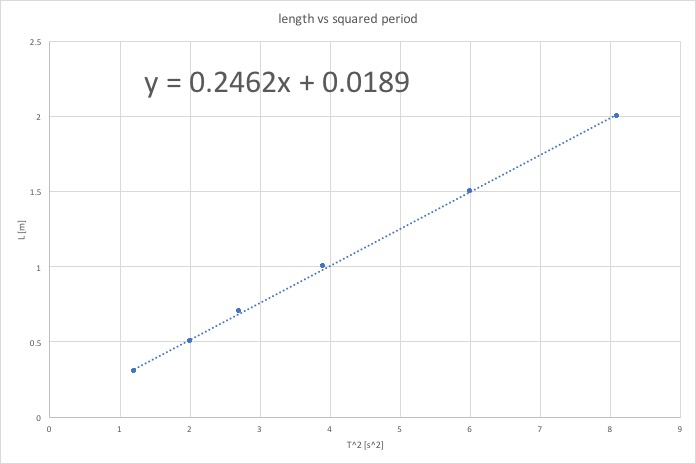
\includegraphics[width=4in]{IntroductionFigures/graph2.jpg}
  \end{center}
  \caption{Example of a graph with the trendline  and the corresponding equation.}
  \label{fig:graph2}
\end{figure}
